% cex-mariadb-racoread.tex

\documentclass{standalone}
% newcommands.tex

\newcommand{\enq}{\texttt{enq}}
\newcommand{\deq}{\texttt{deq}}
\newcommand{\pput}{\texttt{PUT}}
\newcommand{\get}{\texttt{GET}}
\newcommand{\vs}{\texttt{vis}}
\newcommand{\so}{\texttt{so}}
\newcommand{\arb}{\texttt{ar}}
\newcommand{\rf}{\texttt{rf}}

% example
\newcommand{\po}[2]{\draw [->, thick] (#1) to node[above] {\Large{\so}} (#2);}
\newcommand{\pva}[2]{\draw [->, thick] (#1) to node[above] {$\Large{\so},\Large{\vs},\Large{\arb}$} (#2);}
\newcommand{\pbva}[2]{\draw [->, thick] (#1) to node[above] {$\Large{\so}$} node[below] {$\Large{\vs},\Large{\arb}$} (#2);}
\newcommand{\pv}[2]{\draw [->, thick] (#1) to node[above] {\Large{\so}} node[below] {\Large{\vs}} (#2);}
\newcommand{\evis}[2]{\draw [->, thick] (#1) to node[above, sloped, near end] {\Large{\vs}} (#2);}
\newcommand{\mvis}[2]{\draw [->, thick] (#1) to node[above, sloped] {\Large{\vs}} (#2);}
\newcommand{\ar}[2]{\draw [->, thick, allow upside down] (#1) to node[above, sloped] {\Large{\arb}} (#2);}
\newcommand{\va}[2]{\draw [->, thick, allow upside down] (#1) to node[above, sloped] {$\Large{\vs},\Large{\arb}$} (#2);}
\newcommand{\vab}[2]{\draw [->, thick, allow upside down] (#1) to node[below, sloped, near end] {$\Large{\vs},\Large{\arb}$} (#2);}
\newcommand{\vae}[2]{\draw [->, thick, allow upside down] (#1) to node[above, sloped, near end] {$\Large{\vs},\Large{\arb}$} (#2);}
\newcommand{\vas}[2]{\draw [->, thick, allow upside down] (#1) to node[sloped, near start, above] {$\Large{\vs},\Large{\arb}$} (#2);}

% serialization
\newcommand{\scc}[2]{\draw [->, very thick] (#1) to (#2);}
\newcommand{\rva}[2]{\draw [->, thick, allow upside down] (#1) to node[above, sloped] {$\Large{\rf},\Large{\vs},\Large{\arb}$} (#2);}
\newcommand{\rvb}[2]{\draw [->, thick, allow upside down] (#1) to node[below, sloped] {$\Large{\rf},\Large{\vs},\Large{\arb}$} (#2);}


\usepackage{tikz}
\usetikzlibrary{shapes, positioning, arrows.meta, decorations.pathmorphing}

\begin{document}
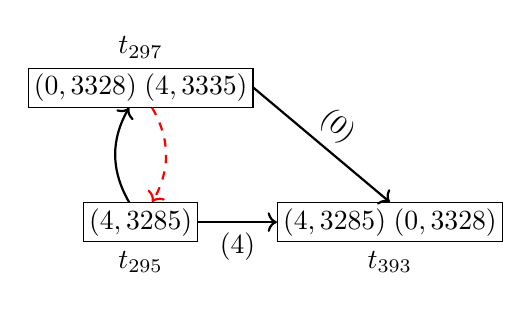
\begin{tikzpicture}[
  so/.style = {->, thick},
  wr/.style = {->, thick},
  co/.style = {->, thick},
  vo/.style = {->, thick},
  txn/.style = {draw, inner sep = 2pt}]

  % t393: R(4, 3285), R(0, 3328)
  \node[txn, label = below : $t_{393}$]
    (t393) {$\readevent(4, 3285) \; \readevent(0, 3328)$};
  % t295: W(4, 3285)
  \node[txn, left = 1.00cm of t393, label = below : $t_{295}$]
    (t295) {$\writeevent(4, 3285)$};
  % t297: W(0, 3328), W(4, 3335)
  \node[txn, above = 1.20cm of t295, label = above : $t_{297}$]
    (t297) {$\writeevent(0, 3328) \; \writeevent(4, 3335)$};

  % t295-WR4-t393
  \draw[wr] (t295) to node[below]{$\WR(4)$} (t393);
  % t295-SO-t297
  \draw[so, bend left] (t295) to node[left]{$\SO$} (t297);
  % t297-WR0-t393
  \draw[wr] (t297.east) to node[sloped, above]{$\WR(0)$} (t393.north);

  % t297-VO-t295
  \draw[vo, dashed, red, bend left] (t297) to node[right]{$\VO$} (t295);
\end{tikzpicture}
\end{document}